In the current section we present the SALSA SCPool. We first show the data structures of SALSA in Section~\ref{alg-structure}, and then present the basic algorithm without stealing support in Section~\ref{alg-overview}. The stealing procedure is described in Section~\ref{alg-stealing}. 
Finally, we argue that SALSA is lock-free~\ref{alg-properties}. 

\subsection{SALSA Structure\label{alg-structure}}
\newcounter{alg:non-fifo:lines}
\begin{algo}[!ht]
\caption{SALSA implementation of SCPool: Data Structures.} 
\label{alg:non-fifo-ds}
\scriptsize
\begin{minipage}[t]{0.48\textwidth}
\begin{distribalgo}[1]
\smallskip

\INDENT {{\bf Chunk type}}
	\STATE Task[CHUNK\_SIZE] tasks 
  \STATE int owner \comment {owner's consumer id}
\ENDINDENT

\INDENT {{\bf Node type}}
  \STATE Chunk c; initially $\bot$
  \STATE int idx; initially -1
  \STATE Node next; 
\ENDINDENT

\setcounter{alg:non-fifo:lines}{\value{ALC@line}} % store the line number
\end{distribalgo}
\end{minipage}%
%
\hfill
%
\begin{minipage}[t]{0.48\textwidth}
%
\begin{distribalgo}[1]
\setcounter{ALC@line}{\value{alg:non-fifo:lines}}
\smallskip

\INDENT {{\bf SALSA per consumer data structure}:}
  \STATE int consumerId
  \STATE List\tup{Node}[] chunkLists \comment {one list per producer + extra list for stealing (every list is single-writer multi-reader)} 
  \STATE Queue\tup{Chunk} chunkPool \comment {pool of spare chunks}
  \STATE Node currentNode, initially $\bot$ \comment {current node to work with} 
\ENDINDENT

\setcounter{alg:non-fifo:lines}{\value{ALC@line}}
\end{distribalgo}
\end{minipage}
\end{algo}


\begin{figure}[htb]
	\centering
	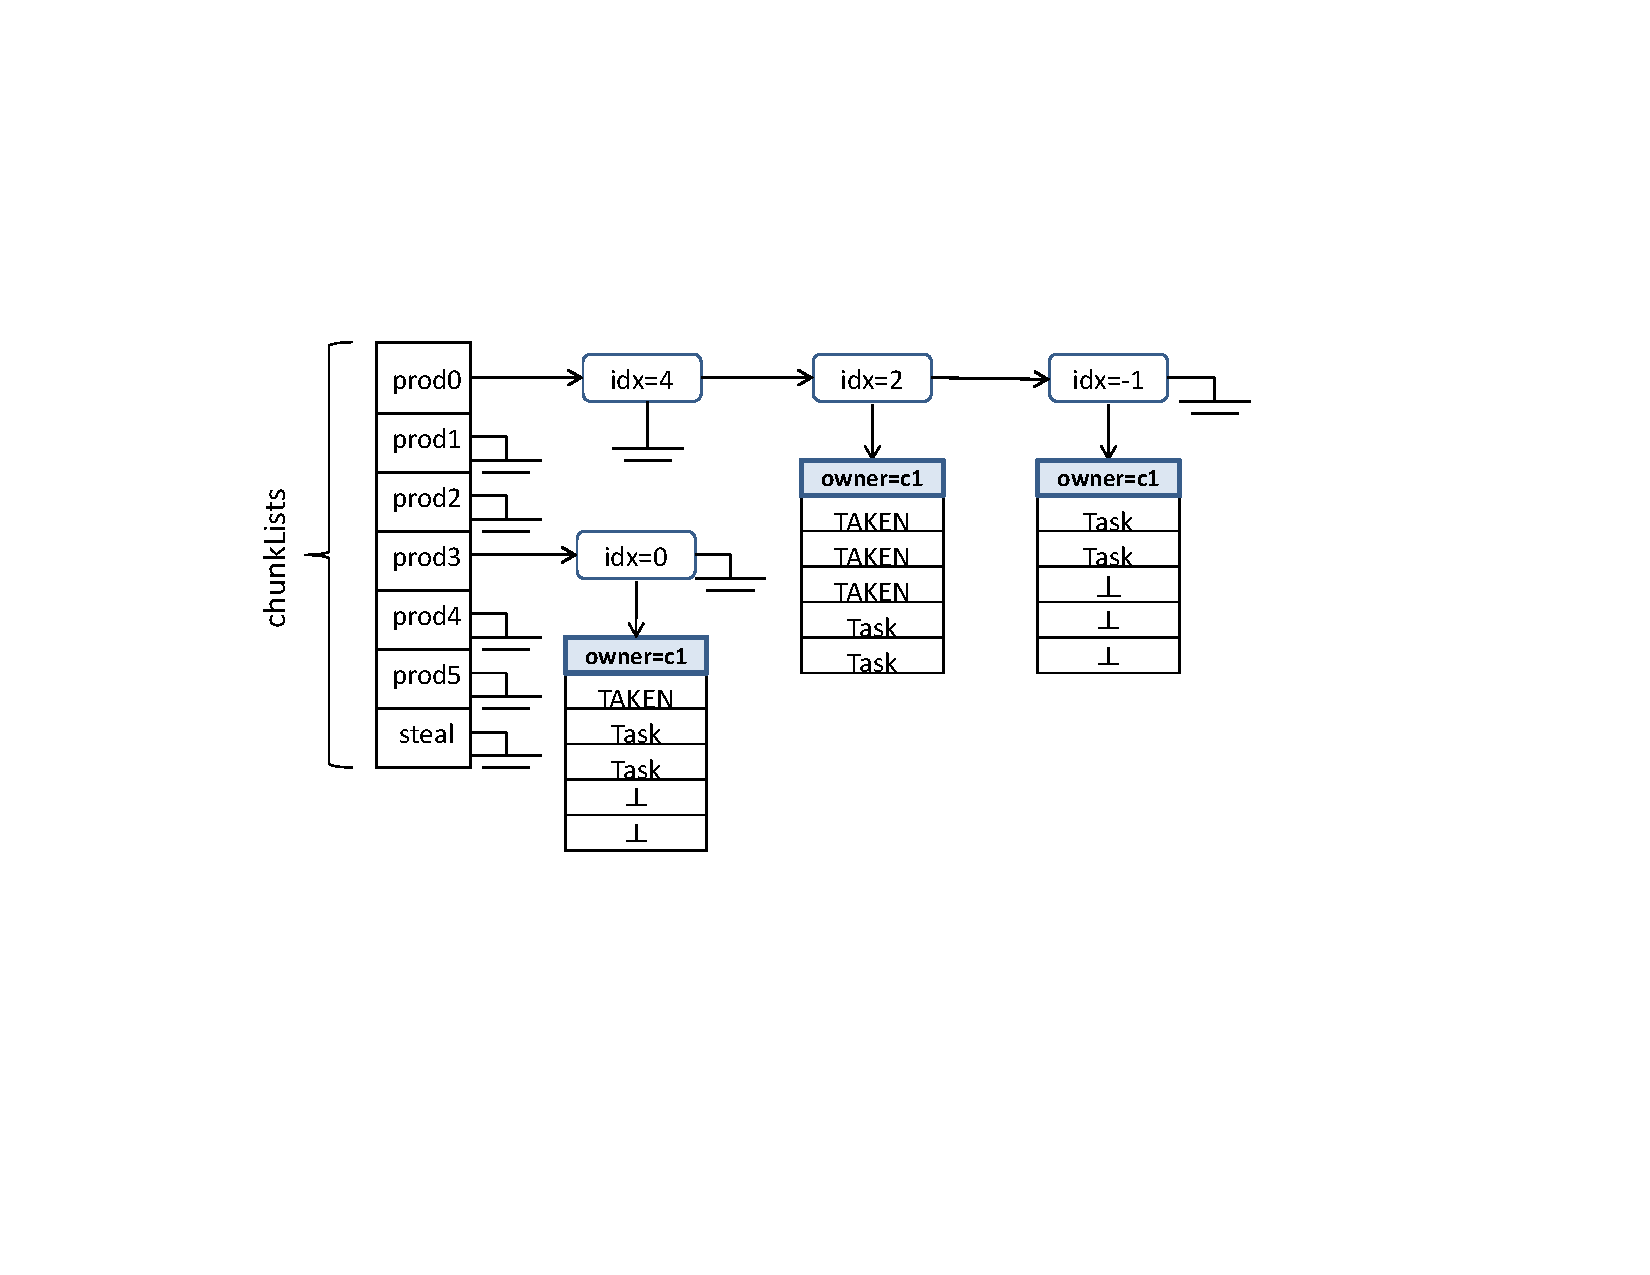
\includegraphics[height=0.3\textwidth]{figures/salsa-struct}
	\caption{
	    \footnotesize{Chunk lists in SALSA single consumer pool implementation. Tasks are kept in chunks, which are 
	    organized in per-producer lists; an additional list is reserved for stealing. Each list can be modified 
	    by the corresponding producer only. The only process that is allowed to retrieve tasks from a chunk is 
	    the owner of that chunk (defined by the ownership flag). A Node's index corresponds to the latest task taken from the chunk
	    or the task that is about to be taken by the current chunk owner. 
	    }}
	\label{fig:salsa-struct}
\end{figure}

We describe the implementation of a SALSA SCPool of some consumer $c_i$.
Its data structures are described in Algorithm~\ref{alg:non-fifo-ds} and partially depicted in Figure~\ref{fig:salsa-struct}. The tasks inserted to SALSA are kept in chunks, which are organized in per-producer chunk lists. Only the producer mapped to a given list can insert a task to any chunk in that list. Every chunk is owned by a single consumer whose id is kept in the \emph{owner} field of the chunk.
The owner is the only process that is allowed to take tasks from the chunk; if another process wants to take a task from the chunk, it should first steal the chunk and change its ownership. The owner of a chunk
residing at $c_i$'s SCPool is $c_i$ itself, unless that chunk is being stolen. A task entry in a chunk is used at most once. It holds the value $\bot$ initially, and TAKEN after the task it held has been consumed.

The per-producer chunk lists are kept in the array \emph{chunkLists} (see Figure~\ref{fig:salsa-struct}), where \emph{chunkLists[j]} keeps a list of chunks with tasks inserted by producer $p_j$. In addition, the array has a special entry \emph{chunkLists[steal]}, holding chunks stolen by $c_i$. Every list has a single writer who can modify the list structure (add or remove nodes), \emph{chunkLists[j]} can be modified only by the producer $p_j$, while the list \emph{chunkLists[steal]} can be modified only by the SCPool's owner $c_i$. Specifically, a consumed node (whose chunk was removed by the consumer) is lazily reclaimed and removed by the list's owner (typically a producer). For brevity, this is omitted from the pseudo-code bellow. Having a single writer allows us to implement the lists without synchronization primitives, similarly to the single-writer linked-list in~\cite{Michael:2004:HPS:987524.987595}.

In addition to the chunk pointer, each node keeps the index of the latest taken task. As we show in Section~\ref{alg-stealing}, this index plays a crucial role in chunk stealing. Safe memory reclamation is provided by using hazard pointers~\cite{Michael:2004:HPS:987524.987595} both for nodes and for chunks.

The free (reclaimed) chunks in SALSA are kept inside the SCPools in \emph{chunkPool}, a lock-free queue~\cite{Michael:1996:SFP:248052.248106}. These pools serve two purposes. First, they enable efficient memory reuse. Second, as we show in Section~\ref{alg-pools}, managing per-consumer chunk pools is good for load balancing. 
\subsection{Algorithm overview\label{alg-overview}}




The local variables and algorithms of the producer appear in
Algorithm~\ref{alg:producer-non-fifo}. The producer's code is fairly simple, the producer first
attempt to add tasks to the chunks it previously used, if this is the first produce action or the
previous chunk was already filled, the producer will attempt to take a chunk from the chunk pool and
add it to its list on the pool of the given consumer. If the pool is empty the operation will fail
with a FULL message, if produceForce was called the operation will not fail, instead a new chunk
will be allocated. 


\subsection{Stealing\label{alg-stealing}}
\subsection{Chunk pools\label{alg-pools}}
\subsection{Lock-freedom\label{alg-properties}}

